\section{Solitario}

\begin{figure}[htbp]
\begin{center}
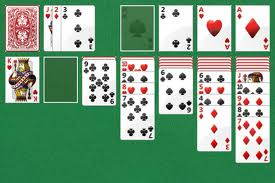
\includegraphics[width=.60\textwidth]{./imagenes/solitario.png}
\caption{Solitario}
\label{Solitario}
\end{center}
\end{figure}
Solitario\footnote{\url{http://solitariospider.org/}} es un juego de naipes o cartas, muy popular en todo el mundo. Precisamente, el nombre se refiere al hecho de que sólo hay un jugador en competencia. Es considerado como un juego de paciencia y destreza cuyo objetivo es utilizar todas las cartas de la baraja para construir las cuatro pilas de naipes clasificadas por pintas comenzando por los ases en orden ascendente.


\subsubsection{¿Por qué es uno de mis juegos favoritos?}
\begin{itemize}
\item Solitario Spider. Consigue emparejar e ir eliminando todas las cartas, formando grupos en funcion de tipo de juego de solitario. Completa en juego limpiando el tablero de cartas y, en algunos casos, antes que se te agote el tiempo.
 
\end{itemize}
